\documentclass{article}
\usepackage[utf8]{inputenc}
\usepackage{graphicx} 
\usepackage{fancyhdr}
\usepackage{ragged2e}
\usepackage{multirow}
\usepackage[hidelinks]{hyperref}
\usepackage[table,xcdraw]{xcolor}
\usepackage{ulem}
\usepackage{listings}
\usepackage[spanish]{babel} % Paquete para idioma español
\usepackage{xcolor} % Para usar colores

\usepackage{caption}

\usepackage{bbding}
\usepackage{pifont}
\usepackage{wasysym}
\usepackage{amssymb}


\definecolor{verdeCompletado}{RGB}{0, 128, 0} % Verde para tareas completadas
\definecolor{azulProgreso}{RGB}{30, 144, 255} % Azul para tareas en progreso
\definecolor{grisPendiente}{RGB}{169, 169, 169} % Gris para tareas pendientes



\usepackage{pgfgantt}
\usepackage{float}
\usepackage{pdflscape} % Paquete para la orientación horizontal
\usepackage{longtable} % Para tablas largas.
\usepackage{geometry} 
\usepackage{ragged2e}
\usepackage{translator}
\ganttset{calendar week text={\small{\startday/\startmonth}}}
\newcommand\textganttbar[5][]{%
    \ganttbar[#1,bar/.append style={alias=tmp}]{#2}{#4}{#5}
    \path 
    let
    \p1=(tmp.west),\p2=(tmp.east),
    \n1={\x2-\x1},\n2={width("#3")},
    \n3={ifthenelse(\n1>\n2,90,270)}
    in
    node [anchor=\n3,font=\footnotesize] at (tmp.north) {#3};
}

% Definir un color azul oscuro
\definecolor{azulOscuro}{RGB}{0, 0, 139} % Azul oscuro


% Adicionales
\addto\captionsspanish{\renewcommand{\contentsname}{Índice}} % Cambio de  Adicionales Contents a Indice
\pagestyle{fancy}
\fancyhf{}
\lhead{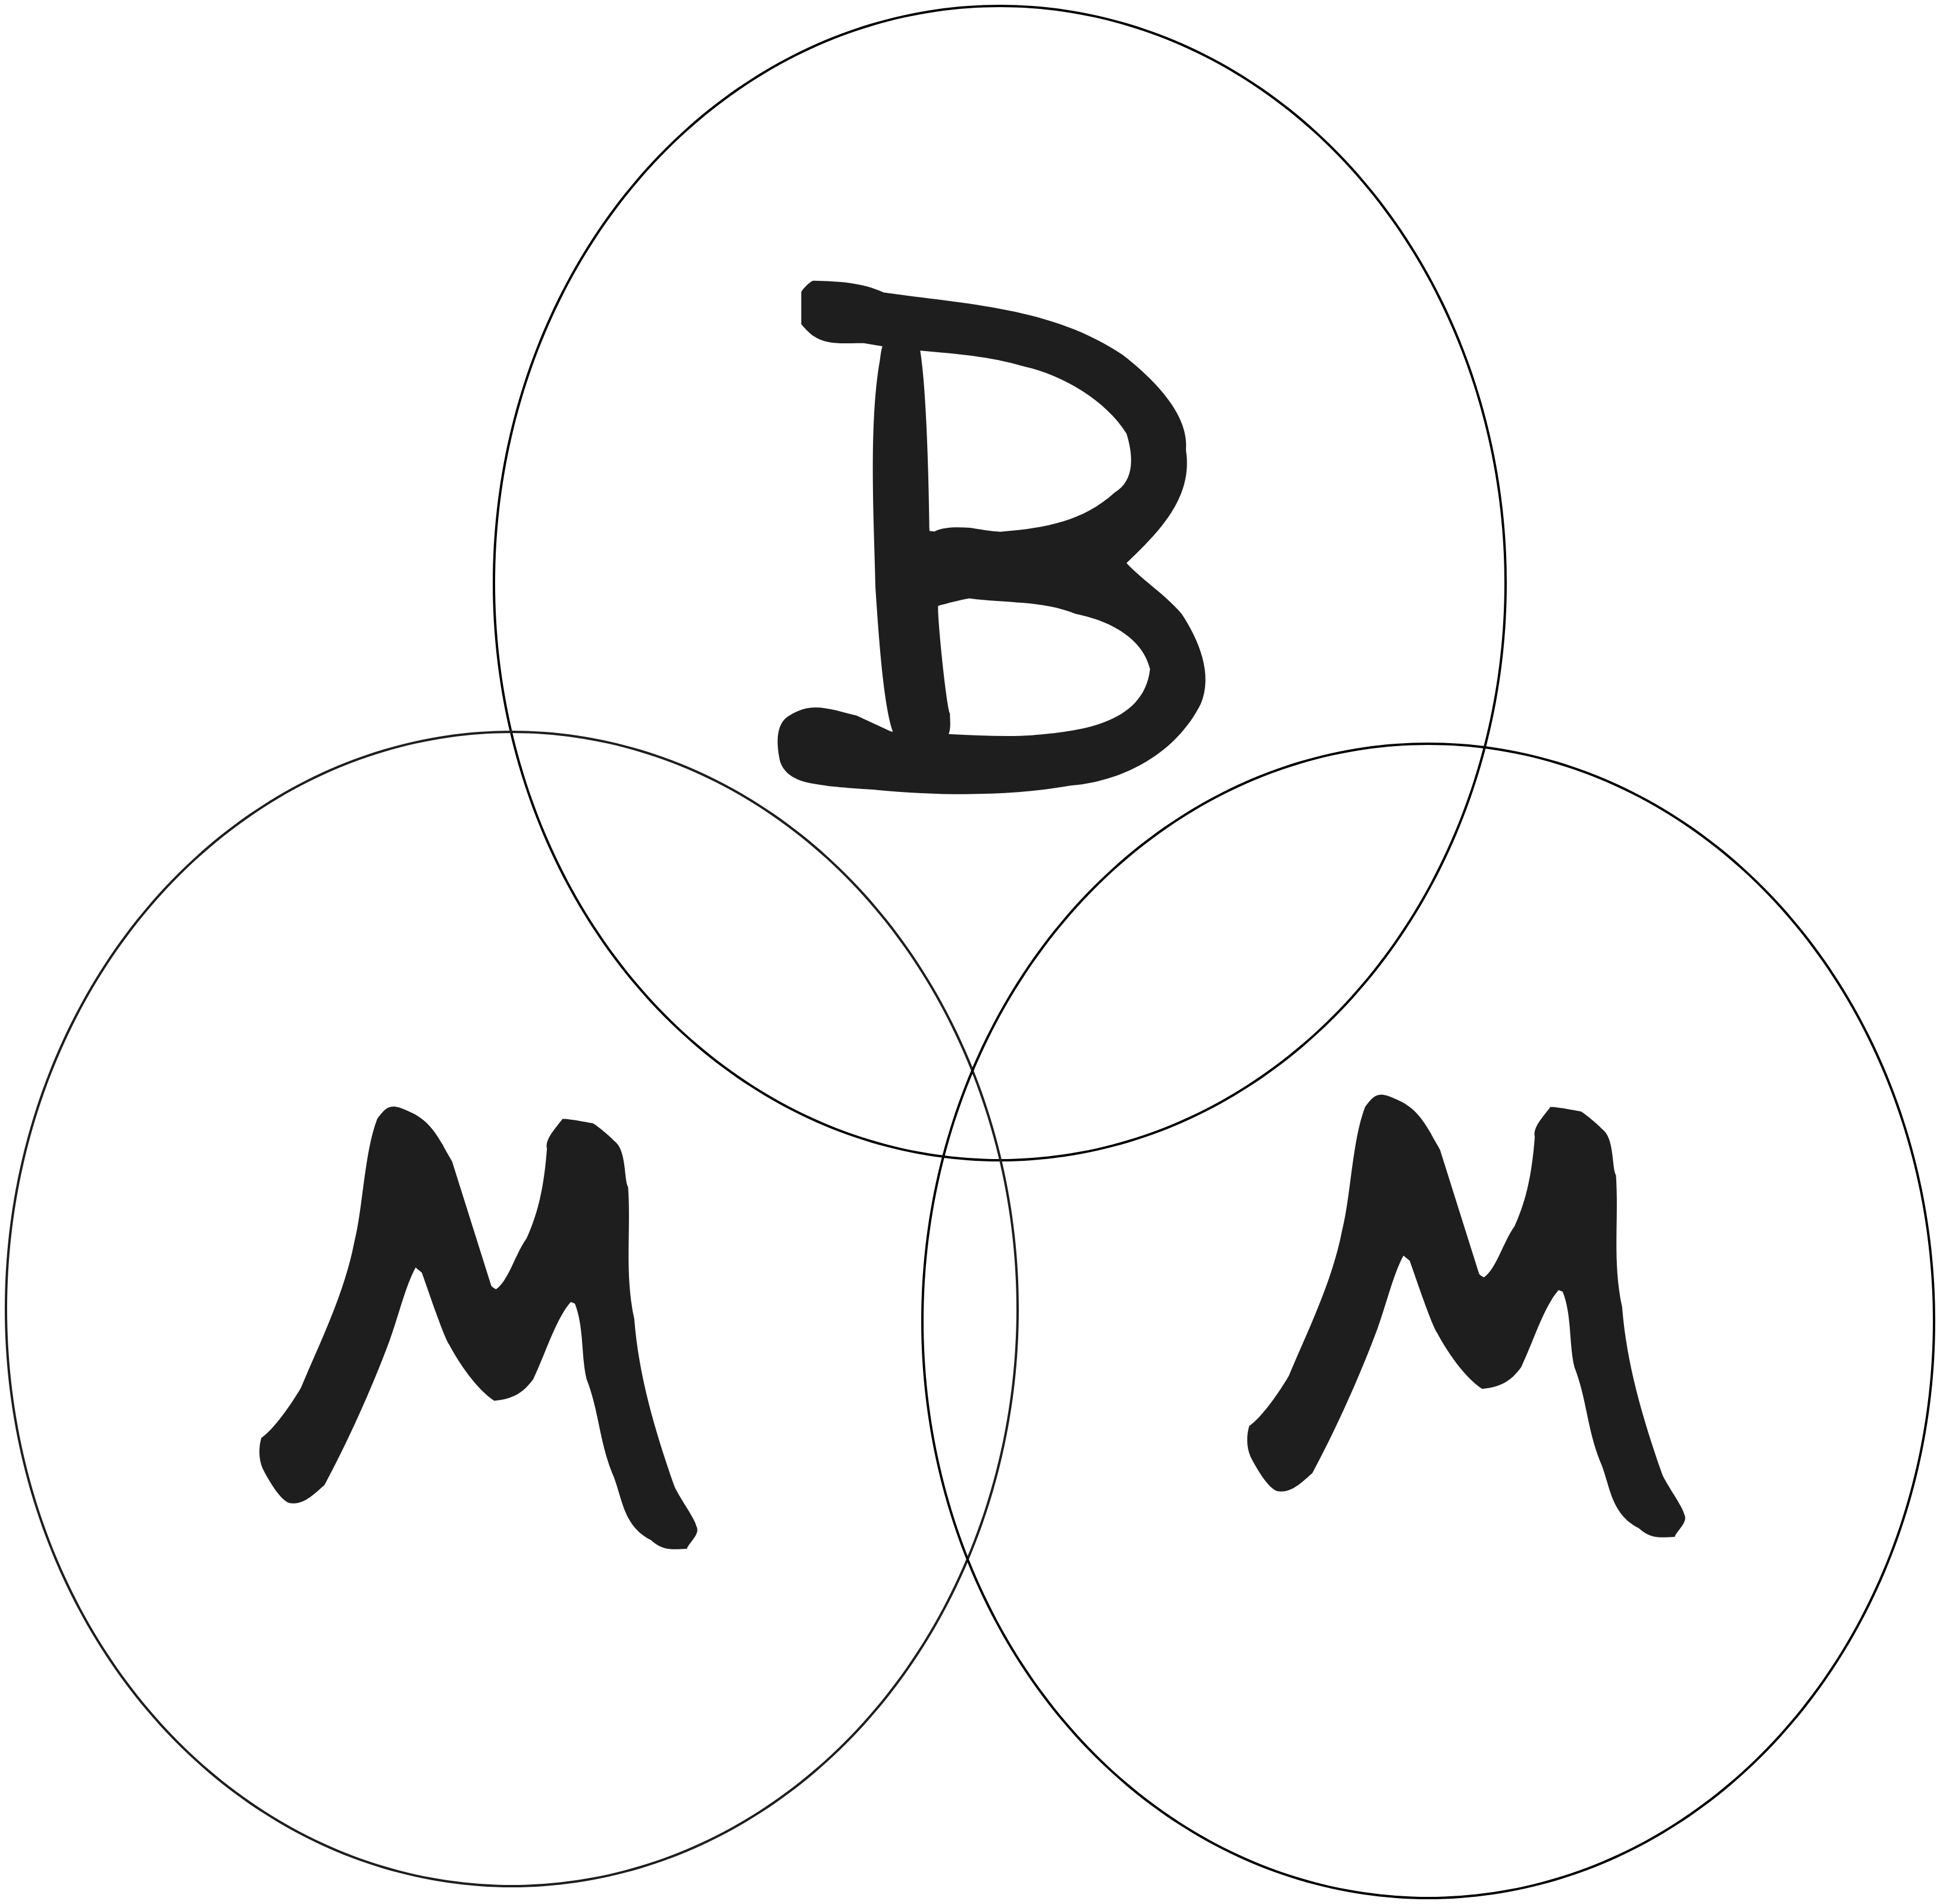
\includegraphics[width=1cm]{TFG/Logo.png}}

\renewcommand{\headrulewidth}{3pt}
   %Comienzo de Documento
    \begin{document}
            % Creacion de Portada----------------------------------------------------------
% Comienzo de Documento
    % Creación de Portada
    \begin{titlepage}
        \begin{center}
            {\scshape\large{Grado Superior}}\\
            {\scshape\large{Desarrollo de aplicaciones multiplataforma}} \\

            
            \vspace{2cm}
            {
\includegraphics[width=0.4\textwidth]{TFG/fotomain.png}} \par
            \vspace{2cm}
            {\scshape\large{ Aplicación para la Gestión de Tareas y Control \\ de Alimentos en el Hogar}\\
            \vspace{2cm}
            \textbf{TaskTracer}}} \\
            \vspace{2cm}
            {\Large Autor:} \\
            \vspace{1mm}
            {\Large Borja Merchán Mckenna} \\
            \vspace{1mm}
            {\Large 08/11/2024}
        \end{center}
    \end{titlepage}

 % ----------------------------------------------------------------
        %Comienzo de Toc
        
        \clearpage
        \tableofcontents

         \clearpage





\section{Prototipo del proyecto}
TaskTracer es una aplicación destinada a la gestión de tareas y control de inventario de alimentos en el hogar, que conecta a los miembros de una familia o grupo de convivencia. A través de la aplicación, los usuarios pueden gestionar sus listas de tareas diarias y controlar el inventario de alimentos en la nevera. La sección de tareas permite a los usuarios añadir, editar y eliminar actividades, mientras que la sección de inventario ayuda a organizar y categorizar productos alimenticios. Además, se realizará la gestión de usuarios y de grupos de hogar para facilitar una administración personalizada dentro de cada grupo.

\section{Entradas, salidas y estados del proyecto}
\begin{itemize}
    \subsection {Entradas del Proyecto}
    \begin{itemize}
        \item \textbf{Datos de Usuario:}
        \begin{itemize}
            \item Registro: Nombre completo, correo electrónico y contraseña para crear una cuenta de usuario.
            \item Inicio de Sesión: Correo electrónico y contraseña para la autenticación.
            \item Opcional: Información adicional del usuario, como la selección de un grupo de hogar.
        \end{itemize}
        
        \item \textbf{Datos de Tareas y Productos:}
        \begin{itemize}
            \item Agregar Tarea: Nombre de la tarea, categoría (personal, trabajo, etc.) y estado de completado.
            \item Agregar Producto: Nombre del producto, categoría (en nevera o por comprar) y ubicación (columnas del tablero Kanban).
        \end{itemize}
        
        \item \textbf{Interacciones de Usuario:}
        \begin{itemize}
            \item Navegación: Selección de botones para navegar entre pantallas (inicio de sesión, registro, grupo de hogar, to-do, nevera, ajustes).
            \item Edición y Organización: Arrastre y cambio de estado de las tareas y productos en los tableros Kanban.
        \end{itemize}
        
        \item \textbf{Configuraciones y Preferencias:}
        \begin{itemize}
            \item Preferencias de Usuario: Elección de un hogar compartido, configuración de grupo o decisión de saltar este paso.
            \item Cierre de Sesión: Elección de cerrar sesión desde la pantalla de ajustes.
        \end{itemize}
    \end{itemize}
    \clearpage
\subsection{Salidas del Proyecto}
    \begin{itemize}
        \item \textbf{Pantallas y Vistas Visuales:}
        \begin{itemize}
            \item Pantallas de Usuario: Confirmación de registro, autenticación exitosa o mensajes de error en caso de fallas en el inicio de sesión.
            \item Tablero de Tareas y Productos: Visualización de tareas pendientes y productos organizados en columnas Kanban.
            \item Detalles de Usuario: Visualización del perfil de usuario, nombre y correo en la pantalla de ajustes.
        \end{itemize}
        
        \item \textbf{Almacenamiento de Datos en Firebase:}
        \begin{itemize}
            \item Información de Usuario: Almacenamiento de los datos de usuario autenticado en Firebase.
            \item Datos de Tareas y Productos: Almacenamiento en Firebase de las tareas creadas y los productos organizados.
        \end{itemize}
        
      
    \end{itemize}

    \subsection{Estados del Proyecto}
    \begin{itemize}
        \item \textbf{Estados de Autenticación:}
        \begin{itemize}
            \item No autenticado: El usuario no ha iniciado sesión y solo puede ver la pantalla de bienvenida y las opciones de autenticación.
            \item Autenticado: El usuario ha iniciado sesión correctamente y puede acceder a todas las funcionalidades de la aplicación.
            \item Sesión Cerrada: El usuario ha salido de su cuenta y vuelve al estado inicial de la aplicación.
        \end{itemize}
        
        \item \textbf{Estados de Navegación:}
        \begin{itemize}
            \item Pantalla de Bienvenida: Estado inicial que guía al usuario a iniciar sesión o registrarse.
            \item Registro y Login: Estado de autenticación donde el usuario se registra o inicia sesión.
            \item Pantalla de Grupo de Hogar: Estado intermedio donde el usuario elige un hogar compartido o decide omitir el paso.
            \item Pantalla Principal (Home): Estado donde el usuario tiene acceso a las pestañas To-Do y Nevera.
            \item Pantalla de Ajustes: Estado donde el usuario puede ver y editar su perfil, además de cerrar sesión.
        \end{itemize}
        
        \item \textbf{Estados de Tareas y Productos:}
        \begin{itemize}
            \item Tarea Activa/Inactiva: Tareas en proceso o completadas, que pueden moverse entre columnas.
            \item Producto en Nevera/Por Comprar: Estado del producto según su columna de Kanban.
        \end{itemize}
        
        \item \textbf{Estado de Configuración del Grupo:}
        \begin{itemize}
            \item Hogar Creado: Indica que el usuario ha creado un hogar.
            \item Hogar Unido: Indica que el usuario se ha unido a un hogar compartido.
            \item Paso Saltado: El usuario ha decidido no crear ni unirse a un hogar.
        \end{itemize}
    \end{itemize}
\end{itemize}



    \section{Planificación completa del proyecto}
    \begin{table}[H]
    \centering
    \begin{tabular}{|l|l|}
        \hline
        \textbf{Clave} & \textbf{Funcionalidades} \\ \hline
         & Inicio de la Aplicación \\ \hline
        F1 & Nombre de la aplicación \\ \hline
        F2 & Logo de la aplicación \\ \hline
        F3 & Investigación de herramientas \\ \hline
         & Diseño de Aplicación \\ \hline
        F4 & Diagrama de Gantt \\ \hline
        F5 & Diagrama de flujo \\ \hline
        F6 & Diseñar en el front \\ \hline
         & Desarrollo \\ \hline
        F7 & Desarrollo de usuarios \\ \hline
        F8 & Desarrollo de grupo de hogar \\ \hline
        F9 & Desarrollo del to-do \\ \hline
        F10 & Desarrollo gestión de nevera \\ \hline
        F11 & Desarrollo de ajustes \\ \hline
         & Implementación en Firebase \\ \hline
        F12 & Implementación de firebase en usuarios \\ \hline
        F13 & Implementación de firebase en grupo de hogar \\ \hline
        F14 & Implementación de firebase en  el to-do \\ \hline
        F15 & Implementación de firebase en  gestión de nevera \\ \hline
        F16 & Implementación de firebase en  ajustes \\ \hline
         & Pruebas y Seguridad \\ \hline
        F17 & Implementación Mejoras  \\ \hline
        F18 & Mantenimiento y Actualización \\ \hline
         & Documentación \\ \hline
        F19 & Documentación en PDF \\ \hline
        F20 & Presentación en PowerPoint \\ \hline
    \end{tabular}
    \caption{Tabla de Funcionalidades}
    \label{tab:funcionalidades}
\end{table}


        \begin{figure}[H]
            \begin{ganttchart}[
            x unit=0.120cm, % distancia entre cada unidad horizontal (días).
            y unit chart=0.5cm, % altura de cada unidad vertical.
            y unit title=0.7cm, % altura de las filas de títulos.
            title height=1, % separación entre una fila de títulos y otra (1 = ninguna separación).
            hgrid, % dibujar las separaciones verticales.
            vgrid={*6{draw=none}, dotted}, % dibujar las separaciones verticales en intervalos semanales.
            bar/.append style={fill=white}, % barras de color blanco por defecto.
            group peaks width=3,
            group peaks tip position=0.5,
            group peaks height=.1, % distintos parámetros para el formato de los grupos.
            time slot format=isodate, % formato de las fechas.
            ] {2024-09-26}{2024-12-15} % inicio y final del eje temporal (año-mes-día).

            % Títulos:
            \gantttitle{Diagrama de Gantt: TaskTracer}{81} \\ % Título centrado y extendido
            \gantttitlecalendar{year, month=shortname} \\ 
            \gantttitlecalendar[title height=2, title label node/.append style={rotate=90}]{week} \\
            \gantttitle[title/.style={opacity=0}]{}{364} \\ 

            % Grupos y tareas:
            \ganttgroup{Inicio de la Aplicación}{2024-09-26}{2024-09-29} \\
            \ganttbar[bar/.append style={fill=blue!20}]{F1  \Large {\CheckedBox}}{2024-09-26}{2024-09-26} \\
            \ganttbar[bar/.append style={fill=blue!20}]{F2  \Large {\CheckedBox}}{2024-09-27}{2024-09-28} \\
            \ganttbar[bar/.append style={fill=blue!20}]{F3  \Large {\CheckedBox} }{2024-09-28}{2024-09-29} \\

            \ganttgroup{Diseño de Aplicación}{2024-09-30}{2024-10-16} \\
            \ganttbar[bar/.append style={fill=orange!50}]{F4 \Large {\CheckedBox}}{2024-09-30}{2024-10-04} \\
            \ganttbar[bar/.append style={fill=orange!50}]{F5 \Large {\CheckedBox}}{2024-10-05}{2024-10-08} \\
            \ganttbar[bar/.append style={fill=orange!50}]{F6 \Large {\CheckedBox}}{2024-10-12}{2024-10-16} \\

            \ganttgroup{Desarrollo}{2024-10-17}{2024-11-20} \\
            \ganttbar[bar/.append style={fill=green!50}]{F7 \Large {\CheckedBox}}{2024-10-17}{2024-10-22} \\
            \ganttbar[bar/.append style={fill=green!50}]{F8 \Large {\CheckedBox}}{2024-10-23}{2024-10-28} \\
            \ganttbar[bar/.append style={fill=green!50}]{F9  \Large {\CheckedBox}}{2024-10-29}{2024-11-03} \\
            \ganttbar[bar/.append style={fill=green!50}]{F10 \Large {\CheckedBox}}{2024-11-04}{2024-11-09} \\
            \ganttbar[bar/.append style={fill=green!50}]{F11 \Large {\CheckedBox}}{2024-11-10}{2024-11-15} \\ 

            
            \ganttgroup{Implementación en Firebase}{2024-10-17}{2024-11-20} \\

       \ganttbar[bar/.append style={fill=green!50}]{F12 \Large {\CheckedBox}}{2024-10-17}{2024-10-22} \\
            \ganttbar[bar/.append style={fill=green!50}]{F13 \Large {\XBox}}{2024-10-23}{2024-10-28} \\
            \ganttbar[bar/.append style={fill=green!50}]{F14 \Large {\XBox}}{2024-10-29}{2024-11-03} \\
            \ganttbar[bar/.append style={fill=green!50}]{F15 \Large {\XBox}}{2024-11-04}{2024-11-09} \\
            \ganttbar[bar/.append style={fill=green!50}]{F16 \Large {\XBox}}{2024-11-10}{2024-11-15} \\

            


             \ganttgroup{Pruebas y Seguridad}{2024-11-20}{2024-12-10} \\
         \ganttbar[bar/.append style={fill=green!50}]{F17 \Large {\XBox}}{2024-11-15}{2024-11-25} \\ 

            \ganttbar[bar/.append style={fill=red!50}]{F18 \Large {\XBox}}{2024-11-20}{2024-12-10} \\ 

            \ganttgroup{Documentación}{2024-11-20}{2024-12-15} \\
            \ganttbar[bar/.append style={fill=green!50}]{F19 \Large {\XBox}}{2024-11-20}{2024-12-15} \\ 
            \ganttbar[bar/.append style={fill=green!50}]{F20 \Large {\XBox}}{2024-12-10}{2024-12-15} \\ 


            % Relaciones de dependencia:

            \end{ganttchart}
            \caption{Diagrama de Gantt de TaskTracer}
            \label{fig:gantt}
        \end{figure}

\section{Prototipo de la aplicación}

\begin{figure}[h!]
    \centering
    \includegraphics[width=0.4\textwidth]{TFG/ciclo de vida/1.png}
    \caption{Imagen 1 del }
\end{figure}

\begin{figure}[h!]
    \centering
    \includegraphics[width=0.4\textwidth]{TFG/ciclo de vida/2.png}
    \caption{Imagen 2 del ciclo de vida de la aplicación}
\end{figure}

\begin{figure}[h!]
    \centering
    \includegraphics[width=0.4\textwidth]{TFG/ciclo de vida/3.png}
    \caption{Imagen 3 del ciclo de vida de la aplicación}
\end{figure}



\begin{figure}[h!]
    \centering
    \includegraphics[width=0.4\textwidth]{TFG/ciclo de vida/4.png}
    \caption{Imagen 4 del ciclo de vida de la aplicación}
\end{figure}

\begin{figure}[h!]
    \centering
    \includegraphics[width=0.4\textwidth]{TFG/ciclo de vida/5.png}
    \caption{Imagen 5 del ciclo de vida de la aplicación}
\end{figure}

\begin{figure}[h!]
    \centering
    \includegraphics[width=0.4\textwidth]{TFG/ciclo de vida/6.png}
    \caption{Imagen 6 del ciclo de vida de la aplicación}
\end{figure}

\begin{figure}[h!]
    \centering
    \includegraphics[width=0.4\textwidth]{TFG/ciclo de vida/7.png}
    \caption{Imagen 7 del ciclo de vida de la aplicación}
\end{figure}

\begin{figure}[h!]
    \centering
    \includegraphics[width=0.4\textwidth]{TFG/ciclo de vida/8.png}
    \caption{Imagen 8 del ciclo de vida de la aplicación}
\end{figure}

 % ----------------------------------------------------------------


\end{document}
